%!TEX root = ../Electrodynamics.tex
\subsection{Волны в круглом металлическом волноводе. Спектр собственных функций и поперечных волновых чисел волн ТЕ и ТМ типов. Структура поля низших типов волн.}


Наиболее часто на практике используются прямоугольные, круглые и коаксиальные волноводы. Займемся изучением круглых волноводов.

\begin{figure}[ht]
	\centering
	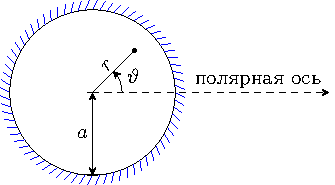
\includegraphics[scale=1.65]{img_lect5/cylindric/geometry}
	\caption{Геометрия круглого волновода}
	\label{fig:cylinder:geometry}
\end{figure}

Область определения задачи $0\leq r \leq a$, $0\leq \vartheta \leq 2\pi$. Каждая точка в сечении волновода задается двумя координатами $(r,\vartheta)$.

Будем решать задачу (пока в общем виде, без граничных условий):
\begin{equation}
	\Delta_\perp \phi+\kappa^2\phi=0
\end{equation}

Здесь лаплассиан в цилиндрических координатах
\begin{equation}
	\Delta_\perp\phi=\frac{1}{r}\pdv{r}\qty(r\pdv{\phi}{r})+\frac{1}{r^2}\pdv[2]{\phi}{\vartheta}
\end{equation}

Также как и при поиске поля в прямоугольном волноводе, воспользуемся методом разделения переменных:
\begin{equation}
	\phi=R(r)\cdot\Theta(\vartheta)
\end{equation}

Применив стандартным образом разделение переменных (подставив $\phi$ как $R\cdot\Theta$ в решаемое уравнение и домножив уравнение слева и справа на $\frac{r^2}{R\Theta}$), получим
\begin{equation}
	\underbrace{r^2\frac{R''}{R}+r\frac{R'}{R}+\kappa^2r^2}_{f(r)=+C_1}+
	\underbrace{\frac{\Theta''}{\Theta}}_{g(\vartheta)=-C_1}
	=0
\end{equation}

Заметим, что комбинация из первых трех слагаемых может зависеть только от $r$, последнее слагаемое может зависеть только от $\vartheta$, а их сумма ни от чего не зависит - значит и первые три слагаемых в сумме ни от чего не зависят и равны некой константе $-C_1$, тогда последнее слагаемое (которое тоже ни от чего не зависит) равно $+C_1$.

Таким образом, разделение переменных успешно завершилось.
\paragraph{Уравнение относительно $\Theta$.}
Такое уравнение запишется в виде
\begin{equation}
	\Theta''+C_1\Theta=0
\end{equation}
Решение этого уравнения (гармонического осциллятора) нам хорошо известно:
\begin{equation}
	\Theta=A_1\cos(\sqrt{C_1}\vartheta)+A_2\sin(\sqrt{C_1}\vartheta)
\end{equation}
Сразу заметим, что отсюда следует, что $\sqrt{C_1}=m$ -- целое число. Действительно, в силу симметрии задачи
\begin{equation}
	\Theta(\vartheta)=\Theta(\vartheta+2\pi),
\end{equation}
а такое возможно только при целой частоте $\sqrt{C_1}$.

\paragraph{Уравнение относительно $r$.} Его можно переписать, если учесть что $\sqrt{C_1}=m$, тогда
\begin{equation}
	R''+\frac{1}{r}R'+\qty(\kappa^2-\frac{m^2}{r^2})R=0
\end{equation}
Можно ввести замену переменных $x=\kappa r$, тогда
\begin{equation}
	R''_{xx}+\frac{1}{x}R'_x+\qty(1-\frac{m^2}{x^2})R=0, \quad R=R(x)
\end{equation}
Это известное уравнение Бесселя. Его решение получается в виде специальных, цилиндрических функций Бесселя:
\begin{equation}
	R=B_q\cdot J_m(x)+B_2\cdot N_m(x)
\end{equation}
$J_m$ называют функциями Бесселя первого рода, или просто функциями Бесселя, а $N_m$ функциями Бесселя второго рода, или функциями Неймана. Их поведение хорошо изучено, не хуже чем поведение синуса и косинуса. Рассмотрим некоторые характерные моменты.
\begin{figure}[ht]
	\centering
	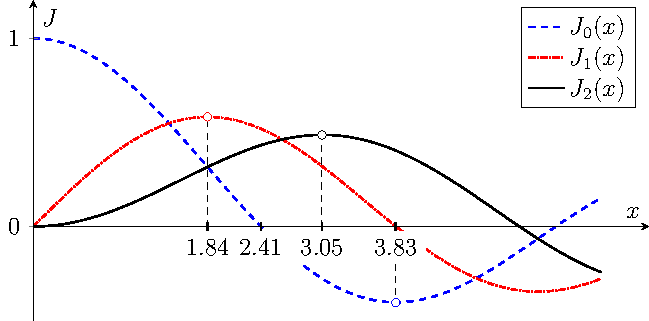
\includegraphics[scale=1.3]{img_lect5/bessel/bessel012}
	\caption{Функции Бесселя первого рода}
	\label{fig:cylinder:besselJ}
\end{figure}
Первый максимум функции Бесселя второго порядка лежит на пересечении функций Бесселя первого и нулевого порядков. Это свойство функций Бесселя. Еще одно свойство заключается в том, что ноль функции Бесселя первого порядка совпадает с точкой минимума функции Бесселя нулевого порядка.
\begin{figure}[ht]
	\centering
	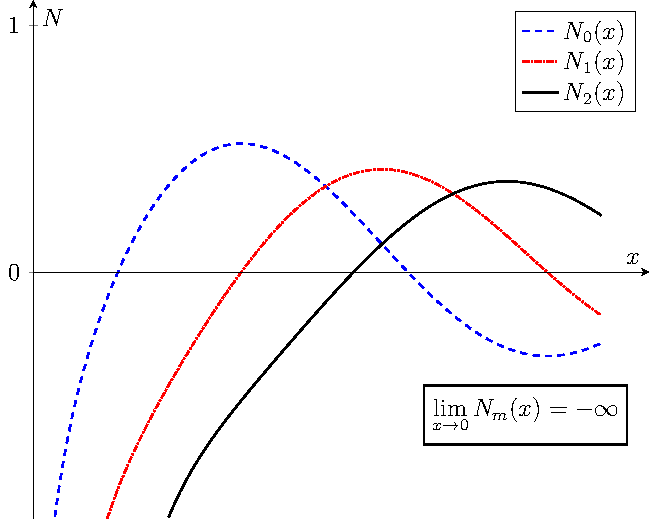
\includegraphics[scale=1.4]{img_lect5/bessel/besselY012}
	\caption{Функции Бесселя второго рода}
	\label{fig:cylinder:besselN}
\end{figure}
Функции Неймана мы пока не будем рассматривать подробно. Это вызвано тем, что у всех функций Неймана есть особенность: в нуле они расходятся, и поэтому в нашем решении, чтобы решение в нуле было конечно, придется положить $B_2=0$.

Вообще говоря, в коаксиальной линии это будет не так, потому что там область определения задачи не включает $r=0$, и  будет $B_2\ne0$.

Итак, наше решение теперь можно переписать в виде
\begin{equation}
	\phi_m=J_m(\kappa r)\qty(A_1\cos(m \vartheta)+A_2\sin(m \vartheta))
\end{equation}
Здесь константу $B_1$ мы уже не пишем, предпологая что она сидит в константах $A_1,A_2$.
Иногда, для краткости, комбинацию синуса и косинуса пишут так:
\begin{equation}
	A_1\cos(m \vartheta)+A_2\sin(m \vartheta)=\mqty(\cos m\vartheta \\\sin m\vartheta)
\end{equation}

Перейдем к удовлетворению граничных условий.

\paragraph{Граничные условия TE-волн.} На границе волновода должна занулятся производная поперечной функции:
\begin{equation}
	\pdv{\phi}{r}\bigg|_{r=a}=0 \quad \Rightarrow \quad \pdv{J_m(\kappa r)}{r}\bigg|_{r=a}=0
\end{equation}
Это значит, что
\begin{equation}
	J_m'(x)=0, \quad x=\kappa a
\end{equation}
Мы можем пронумеровать все нули производной, и обозначить эти точки $x=\mu_{mn}$, где $m$ -- порядок функции Бесселя, а $n$ -- номер нуля производной. Например, $\mu_{11}=1.84$. 
\begin{figure}[H]
	\centering
	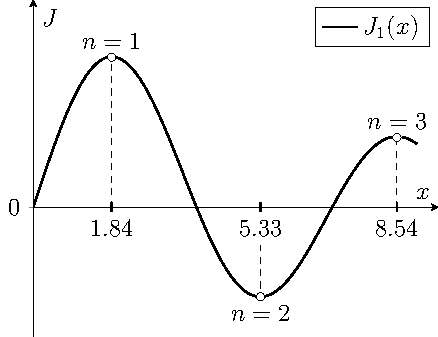
\includegraphics[scale=1.4]{img_lect5/bessel/bessel_mu}
	\caption{Нули производной функции Бесселя}
	\label{fig:cylinder:besselN}
\end{figure}
Тогда можем выразить через $\mu$ и волновое число:
\begin{equation}
	\kappa_{mn}^{TE}=\frac{\mu_{mn}}{a}
\end{equation}
В итоге получаем решение для TE-волн:
\begin{equation}
	\phi_m=C_{mn} J_m(\kappa_{mn} r)\mqty(\cos m\vartheta \\\sin m\vartheta), \quad
	m=0,1,2,3,\ldots \quad n=1,2,\ldots
\end{equation}
Некоторые значения:
\begin{equation}
\begin{aligned}
 		\mu_{11}=&1.84, \quad \kappa_{11}=&\frac{1.84}{a}\\[0.7em]
 		\mu_{21}=&3.05, \quad \kappa_{21}=&\frac{3.05}{a}\\[0.7em]
 		\mu_{01}=&3.83, \quad \kappa_{01}=&\frac{3.83}{a}
\end{aligned} 	
\end{equation} 
\paragraph{Граничные условия TM-волн.} Теперь на границе зануляется поперечная функция:
\begin{equation}
	\phi\big|_{r=a}=0 
		\quad \Rightarrow \quad
			J_m(\kappa r)=0
\end{equation}
Также, как мы это делали для TE-волн, пронумеруем нули функции Бесселя:
\begin{figure}[H]
	\centering
	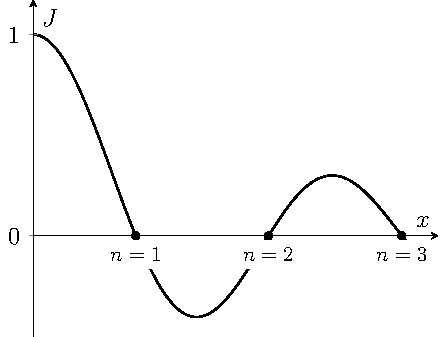
\includegraphics[scale=1.5]{img_lect5/bessel/bessel_kappa}
	\caption{Нули функции Бесселя}
	\label{fig:cylinder:besselN}
\end{figure}
И обозначим нули 
\begin{equation}
	x=\nu_{mn},
\end{equation}
И тогда
\begin{equation}
	\kappa_{mn}^{TM}=\frac{\nu_{mn}}{a}
\end{equation}

Некоторые значения:
\begin{equation}
\begin{aligned}
 		\nu_{01}=&2.405, \quad \kappa_{01}^{TM}=&\frac{2.405}{a}\\[1em]
 		\mu_{11}=&3.83, \quad \kappa_{11}^{TM}=&\frac{3.83}{a}
\end{aligned} 	
\end{equation}

\paragraph{Полное решение задачи.} Если мы введем волновое число как
\begin{equation}
	\kappa_{mn}=\left\{
	\begin{aligned}
		\frac{\mu_{mn}}{a}, \quad \mathrm{TE},\\
		\frac{\nu_{mn}}{a}, \quad \mathrm{TM}
	\end{aligned}\right.
\end{equation}
Тогда полное решение задачи запишется  в виде
\begin{equation}
	\phi_m=C_{mn} J_m(\kappa_{mn} r)\mqty(\cos m\vartheta \\\sin m\vartheta), \quad
	m=0,1,2,3,\ldots \quad n=1,2,\ldots
\end{equation}
\paragraph{Низшая мода.} У низшей моды наименьшее волновое число. В случае круглого волновода низшей модой будет TE$_{11}$: $\kappa_{11}=\frac{1.84}{a}$.
\begin{figure}[H]
	\centering
	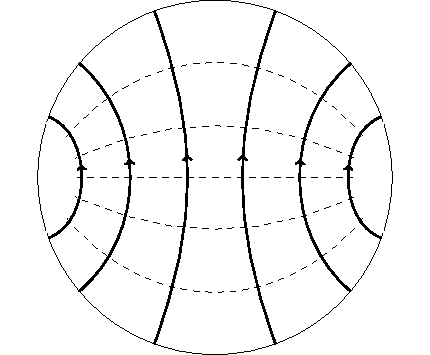
\includegraphics[scale=1.4]{img_lect5/cylindric/TE11}
	\caption{Электрическое и магнитное поле в волне TE$_{11}$}
	\label{fig:cylinder:TE11}
\end{figure}
\paragraph{Замечание.} Можно сформулировать некоторое правило рисования силовых линий. Если построить линии уровня $\phi=\mathrm{const}$, то это будут силовые линии чисто поперечного поля.

Вообще говоря, поле моды TE$_{11}$ круглого волновода топологически подобно моде TE$_{10}$ прямоугольного волновода. Если постепенно деформировать стенки прямоугольного волновода, скругляя их, то линии поля постепенно будут переходить в линии поля круглого волновода.

Кроме того, мода TE$_{11}$ круглого волновода \textbf{двукратно вырождена:} имеет место так называемое \textbf{поляризационное вырождение}.
 
Действительно, если повернуть волновод на 90 градусов, то получаем другое решение. Их не бесконечно много, а всего два фундаментальных, а все остальные образуются как их суперпозиция. 

\subsection{Метод решения задачи о возбуждении идеального полого резонатора сторонними переменным токами. Потенциальные и вихревые поля. Ортогональность полей собственных мод}

Будем решать задачу, пользуясь разложением поля по собственным модам резонатора
$\qty{\vec{E}_p(\vec{r}\,),\vec{H}_p(\vec{r}\,)}\cdot e^{i\omega_p t}$, где 
$p=1,2,3, \ldots$.
\begin{equation}
    \Rot \vec{H}_p = \frac{i\omega_p}{c}\varepsilon \vec{E}_p, \quad
    \Rot \vec{E}_p = -\frac{i\omega_p}{c}\mu \vec{H}_p
\end{equation}
Тогда полное поле можно представить как суперпозицию полей собственных мод. Кроме того, учтём, что $\Div\qty{\vec{E}_p,\vec{H}_p}=0$, тогда можем прибавить еще и потенциальные поля:
\begin{equation}
    \label{eq:EH}
    \vec{E} = \sum\limits_{p = 0}^{\infty} e_p \vec{E}_p + \vec{E}_\text{п}, \quad
    \vec{H} = \sum\limits_{p = 0}^{\infty} h_p \vec{H}_p +\vec{H}_\text{п}
\end{equation}

Докажем свойство \textbf{ортогональности полей собственных мод}. Для этого воспользуемся векторным тождеством:
\begin{equation}
    \Div \qty[\vec{E}_p \times \vec{H}_q\,]=
    \vec{H}_q \Rot \vec{E}_p - \vec{E}_p \Rot \vec{H}_q
\end{equation}
Теперь подставим сюда выражения роторов из уравнений Максвелла:
\begin{equation}
    \Div \qty[\vec{E}_p \times \vec{H}_q\,]=
    \vec{H}_q \qty(-\frac{i\omega_p}{c}\mu \vec{H}_p)-
    \vec{E}_p \qty(\frac{i\omega_p}{c}\varepsilon \vec{E}_p)
\end{equation}
Проинтегрируем левую и правую части равенства по объёму резонатора и воспользуемся теоремой Остроградского-Гаусса:
\begin{equation}
    \oint\limits_S\qty[\vec{E}_p, \vec{H}_q\,] \vec{n} \dd S =
    \int\limits_V\qty[
        \mu \omega_p \vec{H}_p \vec{H}_q + \varepsilon \omega_q \vec{E}_p \vec{E}_q
    ] \dd V
\end{equation}
Заметим, что в левой части стоит ноль, так как $\qty[\vec{E}_p, \vec{H}_q]\equiv\qty[\vec{E}_{\tau_p},\vec{H}_q\,]=0$. Тогда введя обозначения $a=\int \mu \vec{H}_q \vec{H}_p \dd V$, $b=\int \varepsilon \vec{E}_q \vec{E}_p \dd V$, получим систему уравнений
\begin{equation}
    \left\{\begin{aligned}
        \omega_p a + \omega_q b=0\\
        \omega_q a + \omega_p b = 0
    \end{aligned}\right.
\end{equation}
Отсюда видно, что $a,b \ne 0$, когда определитель системы ноль -- значит, если нет вырождения, то $\omega_p=\omega_q$ ($q=p$), а $a=-b$. Это и есть условие ортогональности: интеграл по объёму от произведения полей мод не равен нулю, только если они совпадают.

Введём понятие \textbf{нормы моды}:
\begin{equation}
    N_p = \frac{1}{4\pi} \int\limits_V \varepsilon \qty(\vec{E}_p)^2 \dd V=
    -\frac{1}{4\pi}\int\limits_V \mu \qty(\vec{H}_p)^2 \dd V
\end{equation}

Теперь займёмся подставкой полученных результатов в уравнения Максвелла. Запишем их в случае гармонических полей:
\begin{equation}
    \left\{\begin{aligned}
            &\Rot \vec{E} =  -\frac{i\omega \mu}{c} \vec{H} - \frac{4\pi}{c}\vec{j}^m\\
            &\Rot \vec{H} =  \frac{i\omega\varepsilon}{c} \vec{E} + \frac{4\pi}{c}\vec{j}^e
    \end{aligned}\right.
\end{equation}
Отсюда получается
\begin{equation}
    \left\{\begin{aligned}
      &\sum\limits_{p = 0}^{\infty} e_p \Rot \vec{E}_p + \xcancel{\Rot \vec{E}_\text{п}}=
   - \frac{i\omega \mu}{c} \qty(\sum h_p \vec{H}_p + \vec{H}_\text{п})-\frac{4\pi}{c}\vec{j}^m
            \\             
      &\sum\limits_{p = 0}^{\infty} h_p \Rot \vec{H}_p + \xcancel{\Rot \vec{H}_\text{п}}=
    \frac{i\omega \varepsilon}{c} \qty(\sum e_p \vec{E}_p + \vec{E}_\text{п})+\frac{4\pi}{c}\vec{j}^e
    \end{aligned}\right.
\end{equation}
Наконец, подставим выражения для $\Rot \vec{E}_p, \Rot \vec{H}_p$:
\begin{equation}
    \left\{\begin{aligned}
      &\sum\limits_{p = 0}^{\infty} e_p \qty(-\frac{i\omega_p \mu}{c} \vec{H}_p) =
   - \frac{i\omega \mu}{c} \qty(\sum h_p \vec{H}_p + \vec{H}_\text{п})-\frac{4\pi}{c}\vec{j}^m
            \\             
      &\sum\limits_{p = 0}^{\infty} h_p \qty(\frac{i\omega_p \varepsilon}{c} \vec{E}_p)=
    \frac{i\omega \varepsilon}{c} \qty(\sum e_p \vec{E}_p + \vec{E}_\text{п})+\frac{4\pi}{c}\vec{j}^e
    \end{aligned}\right.
\end{equation}
Перепишем полученные выражения в более удобном виде:
\begin{equation}
    \label{eq:oeoe}
    \left\{\begin{aligned}
            &-i\varepsilon \sum\limits_p \qty(\omega e_p - \omega_p h_p)\vec{E}_p = 4\pi \vec{j}^e + i\omega \varepsilon \vec{E}_\text{п}\\ 
            &-i\mu \sum\limits_p \qty(\omega_p e_p - \omega h_p)\vec{H}_p = -4\pi \vec{j}^m - i\omega \mu \vec{H}_\text{п}
    \end{aligned}\right.
\end{equation}
Возьмём дивергенцию от левой и правой частей равенств \eqref{eq:oeoe}. Левая часть обратится в ноль, так как $\vec{E}_p, \vec{H}_p$ -- вихревые поля, и тогда
\begin{equation}
    \Div \qty(\varepsilon \vec{E}_\text{п}) = -\frac{4\pi}{i\omega} \Div \vec{j}^e,\quad
    \Div \qty(\mu \vec{H}_\text{п}) = -\frac{4\pi}{i\omega} \Div \vec{j}^m
\end{equation}
Зададим потенциальные поля через функции потенциала:
\begin{equation}
    \vec{E}_\text{п} = -\Grad \varphi^e, \quad
    \vec{E}_\text{п} = -\Grad \varphi^m
\end{equation}
Тогда в изотропном случае (когда $\varepsilon,\mu$ можно вытащить из-под дивергенции) получим, с учётом уравнения непрерывности ($\pdv{t}\rho=i\omega \rho = -\Div \vec{j}$):
\begin{equation}\label{eq:pot}
    \Delta \varphi^e = -\frac{4\pi}{\varepsilon} \rho^e, \quad
    \Delta \varphi^m = -\frac{4\pi}{\mu} \rho^m
\end{equation}
Граничные условия найдутся из полей: 
\begin{equation}
   \vec{E}_\tau=0 \Rightarrow \varphi^e\bigg|_S=0, \quad
   H_n=0 \Rightarrow \pdv{\varphi^m}{n}\bigg|_s=0 
\end{equation}

Теперь займёмся нахождением коэффициентов в разложении по собственным модам. Для этого домножим первое уравнение системы \eqref{eq:oeoe} на $\vec{E}_q$, второе на $\vec{H}_q$ и проинтегрируем по области резонатора. В силу ортогональности сумма выродится в одно слагаемое с $q=p$. 
Заметим, что интегралы $\int \vec{E}_\text{п} \vec{E}_q \dd V = 0$ и тоже самое для поля $\vec{H}$. Это нетрудно доказать самим. После несложных преобразований получим
\begin{gather}\label{ga:vih}
    e_p = \frac{i}{\omega^2-\omega_p^2} \frac{1}{N_p}
    \int\limits_V \qty(\omega \vec{j}^e \vec{E}_p - \omega_p \vec{j}^m \vec{H}_p) \dd{V}, \\
 h_p = \frac{i}{\omega^2-\omega_p^2} \frac{1}{N_p}
    \int\limits_V \qty(\omega_p \vec{j}^e \vec{E}_p - \omega \vec{j}^m \vec{H}_p) \dd{V}
\end{gather}

Итак, мы решили задачу о возбуждении токами в резонаторе. При этом поле получилось
суммой двух полей: вихревого и потенциального. Вихревое мы находим как ряд, коэффициенты которого находятся интегрированием \eqref{ga:vih}. Потенциальное же находится через решение уравнения Пуассона на потенциалы \eqref{eq:pot}. А результирующее возбуждённое поле запишется в виде
 \eqref{eq:EH}.
